\begin{figure}[t]
\centering
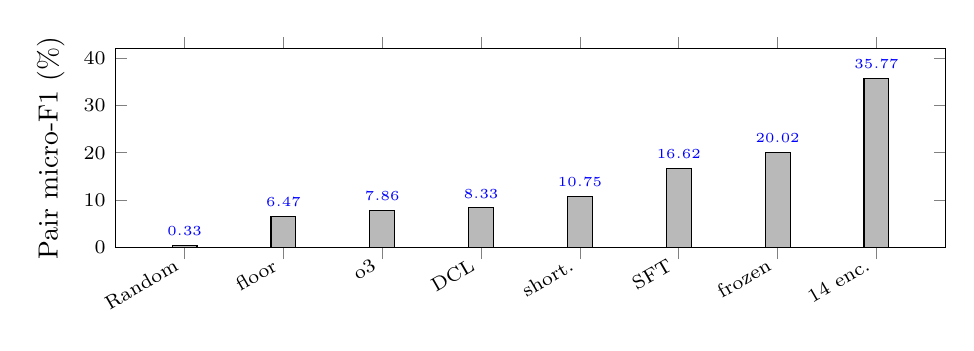
\begin{tikzpicture}
\begin{axis}[ybar,width=\columnwidth,height=4.1cm,bar width=9pt,ymin=0,ymax=42,ylabel={Pair micro-F1 (\%)},symbolic x coords={1,2,3,4,5,6,7,8},
 xtick=data,xticklabels={Random,floor,o3,DCL,short.,SFT,frozen,14 enc.},tick label style={font=\scriptsize},nodes near coords,nodes near coords style={font=\tiny},x tick label style={rotate=30,anchor=east}]
\addplot+[fill=gray!55,draw=black] coordinates {(1,0.33) (2,6.47) (3,7.86) (4,8.33) (5,10.75) (6,16.62) (7,20.02) (8,35.77)};
\end{axis}
\end{tikzpicture}
\caption{AEGIS-Bench, authors' file: published rows (Random, o3, DCL, Aegis-SFT), our trivial floor, shortcut-only (no text), frozen-encoder model and the 14-encoder ensemble.}
\label{fig:aegis}
\end{figure}
